\begin{frame}{``Business Cycle Anatomy'' Setup}
    
    \label{replication-slide}

    VAR with 10 variables, 1955 to 2017

    \vspace{0.5cm}

    \textbf{Identification scheme:}

    Choose the linear combination of empirically estimated reduced-form VAR residuals that explains most of the forecast error variance in a target variable, at a target frequency.

    \vspace{0.5cm}

    \textbf{Initial Target:}
    \begin{itemize}
        \item Business cycle frequency: $\left(\frac{2\pi}{32}, \frac{2\pi}{6}\right)$
        \item Unemployment
    \end{itemize}
    
    
\end{frame}


\begin{frame}{Forecast Error Variance Maximization}

    \begin{figure}
        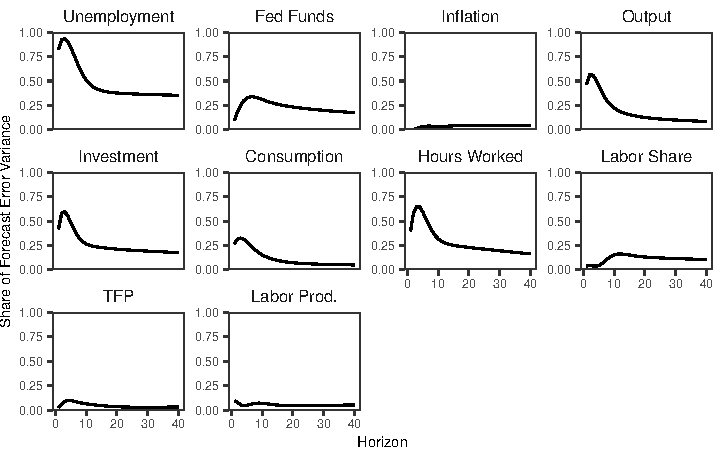
\includegraphics[height = 3in]{figs/fig0_bca_fevd_rep.pdf}
    \end{figure}

\end{frame}


\begin{frame}{Replication of ``Business Cycle Anatomy''}

    \begin{figure}
        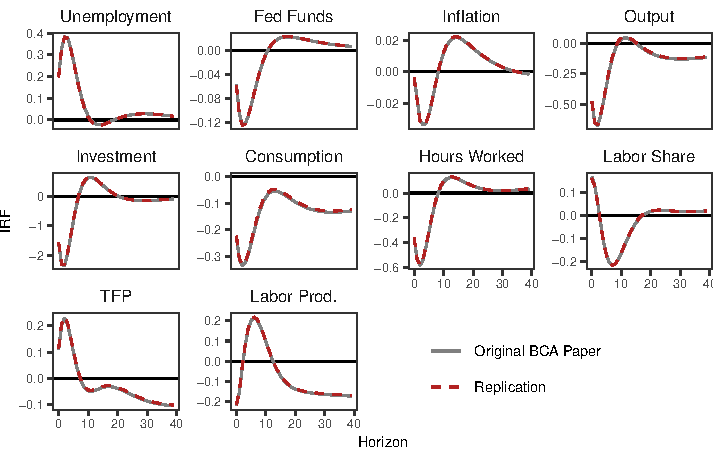
\includegraphics[height = 3in]{figs/fig1_bca_replication.pdf}
    \end{figure}

\end{frame}
